\section{Experiment Design}

To ensure experimental validity, all intermediate evaluation and hyperparameter tuning was performed on $23$ randomly selected images that were separate from both training image set of $106$ images and the final test set of $23$ images. All examples and images are taken from the evaluation set, with final metrics being taken on the test set. No results are taken from the train set, as they would have little meaning.

\section{Existing Pipelines}

To attempt to generate a baseline to assess new methods against, Tesseract \cite{SmithTesseract}, a popular OCR engine sponsored by Google \cite{Vincent} and Ocular \cite{Berg-Kirkpatrick}, another OCR engine based on stochastic models, were integrated into the pipeline using pytesseract \cite{Lee} and by calling jar files from python respectively.

\subsection{Evaluation Metrics}

As these existing pipelines were assessed in the early phases of the project, a full ground truth to evaluate them on was not yet generated as the bounding of lines was not fully implemented. Therefore, they were assessed on how well they were able to detect the quantity of glyphs in an image and how visually close the transcriptions looked when the images were looked at by a human. These metrics proved to be enough to evaluate the methods as both methods were far enough away from an acceptable solution that a more exact metric for comparison was not needed.

\subsection{Tesseract}

With Tesseract, using the ancient Greek corpus, and using both raw and binarized images, the output was comparable to noise, with the transcription lengths being an order of magnitude different from the ground truths.

\subsection{Ocular}
\todo{NEW}

Similarly, training Ocular on both raw and binarized full images and individual glyph images, the output was comparable to noise, with the transcription lengths being an order of magnitude different from the ground truths and $A$ and $\Lambda$ making up over $95\%$ of the returned glyphs. This result happened regardless of the dataset that Ocular was trained on, with binarized and non-binarized images performing the same and singular glyph images performing the same as whole images.

\section{Binarization}

\subsection{Evaluation Metrics}

As there was no ground-truth information provided to compare binarizations against, visual comparison was utilized to determine which binarization method was providing the highest quality binarizations. This was done on four different images, which contained various features that would allow for quick visual evidence of the effectiveness of the methods \seefig{binarizationRaw}. The four images are of assorted sizes, from different collections, and are degraded to different degrees, allowing them to function as a valuable quick assessment tool without introducing bias into the evaluation of the methods.

To assess each binarization method, these images were used to determine how much of the ink on the papyrus was being included, and if noise was being added to the image in the form of background pixels being black or ink pixels being white. This metric was designed to ensure that the signal-to-noise ratio would be low and that the recall and precision would be high, even if they were not directly measurable without a ground truth for each pixel.

\begin{figure}[H]
    \caption{Four Images Utilized to Visually Assess Binarization Quality}
    \label{fig:binarizationRaw}
    \begin{center}
        \begin{subfigure}[b]{0.45\textwidth}
            \centering
            \caption{Example File A}
            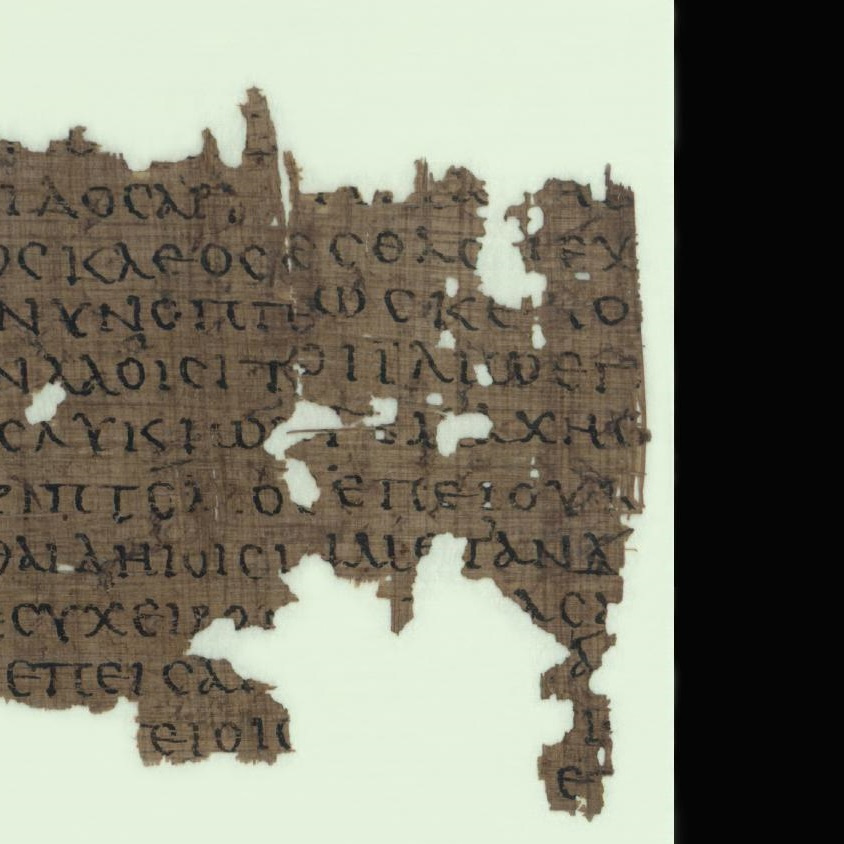
\includegraphics[width=\textwidth]{{raw/G_02317_26742_Pap_crop.jpg}}
        \end{subfigure}
        \hfill
        \begin{subfigure}[b]{0.45\textwidth}
            \centering
            \caption{Example File B}
            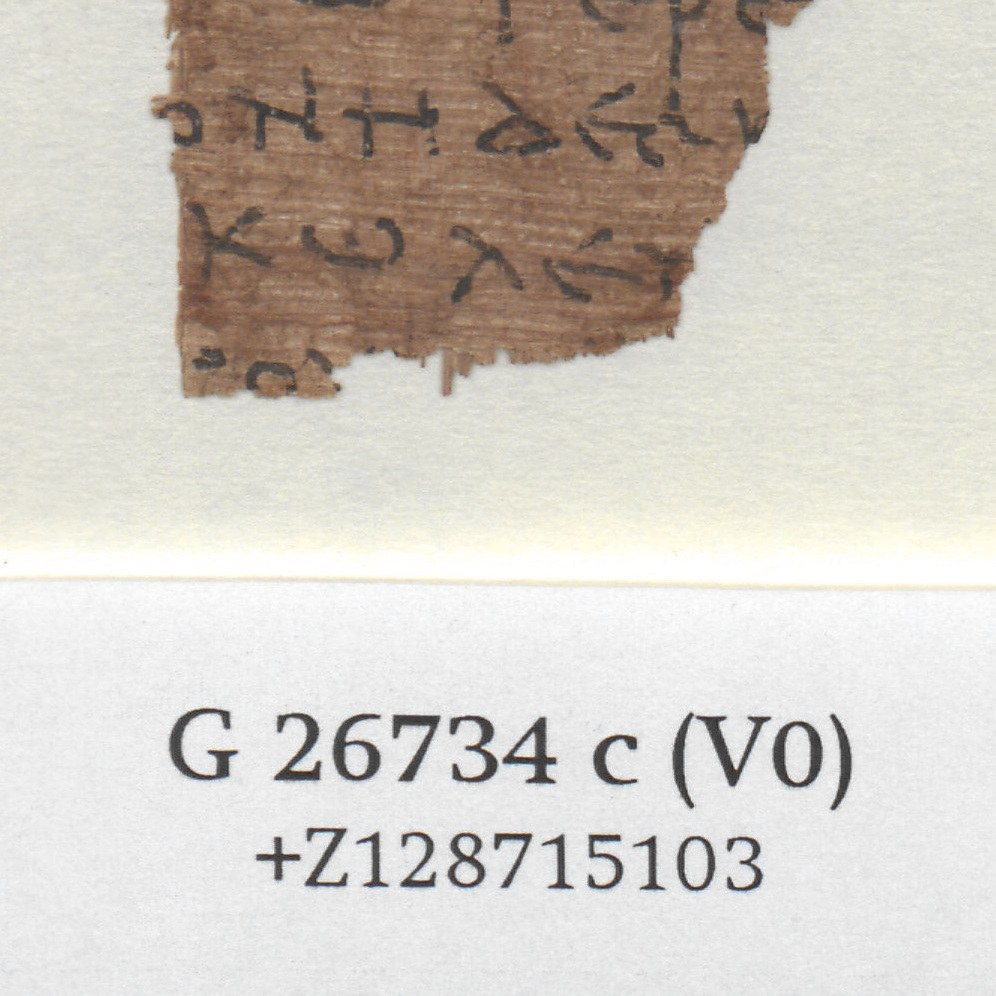
\includegraphics[width=\textwidth]{{raw/G_26734_c_crop.jpg}}
        \end{subfigure}
        \vfill
        \begin{subfigure}[b]{0.45\textwidth}
            \centering
            \caption{Example File C}
            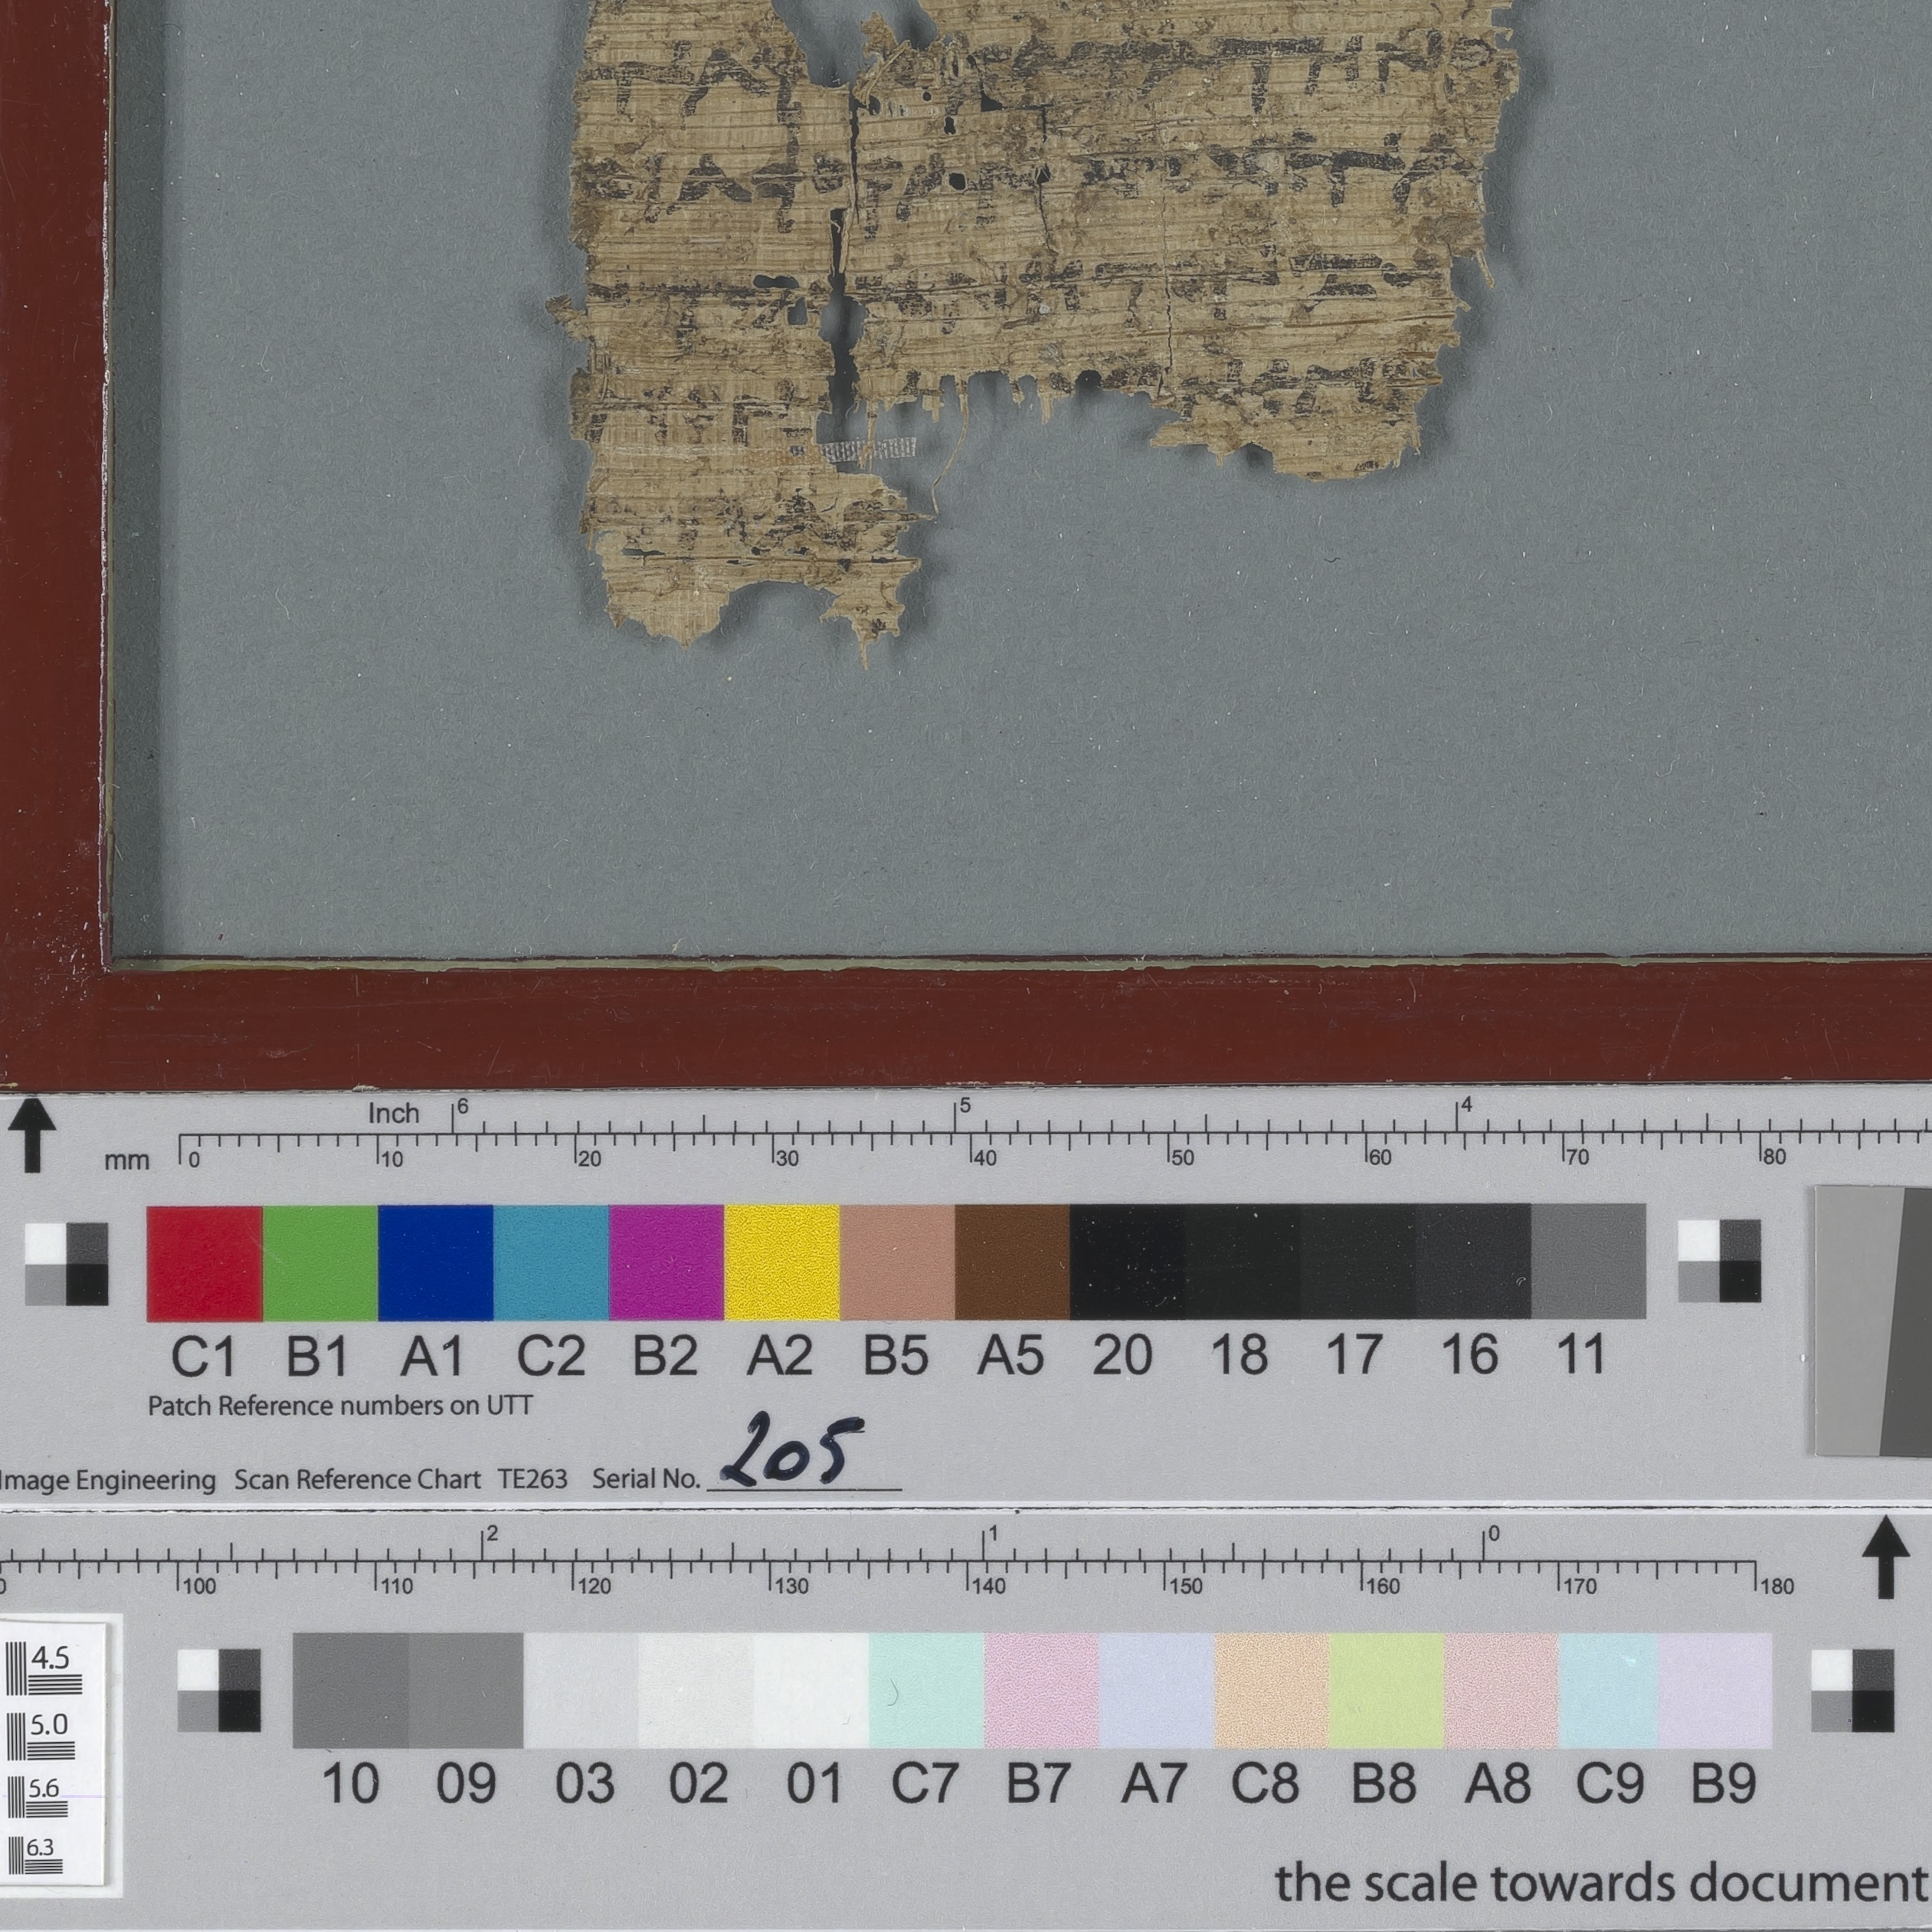
\includegraphics[width=\textwidth]{{raw/P_Hamb_graec_665_crop.jpg}}
        \end{subfigure}
        \hfill
        \begin{subfigure}[b]{0.45\textwidth}
            \centering
            \caption{Example File D}
            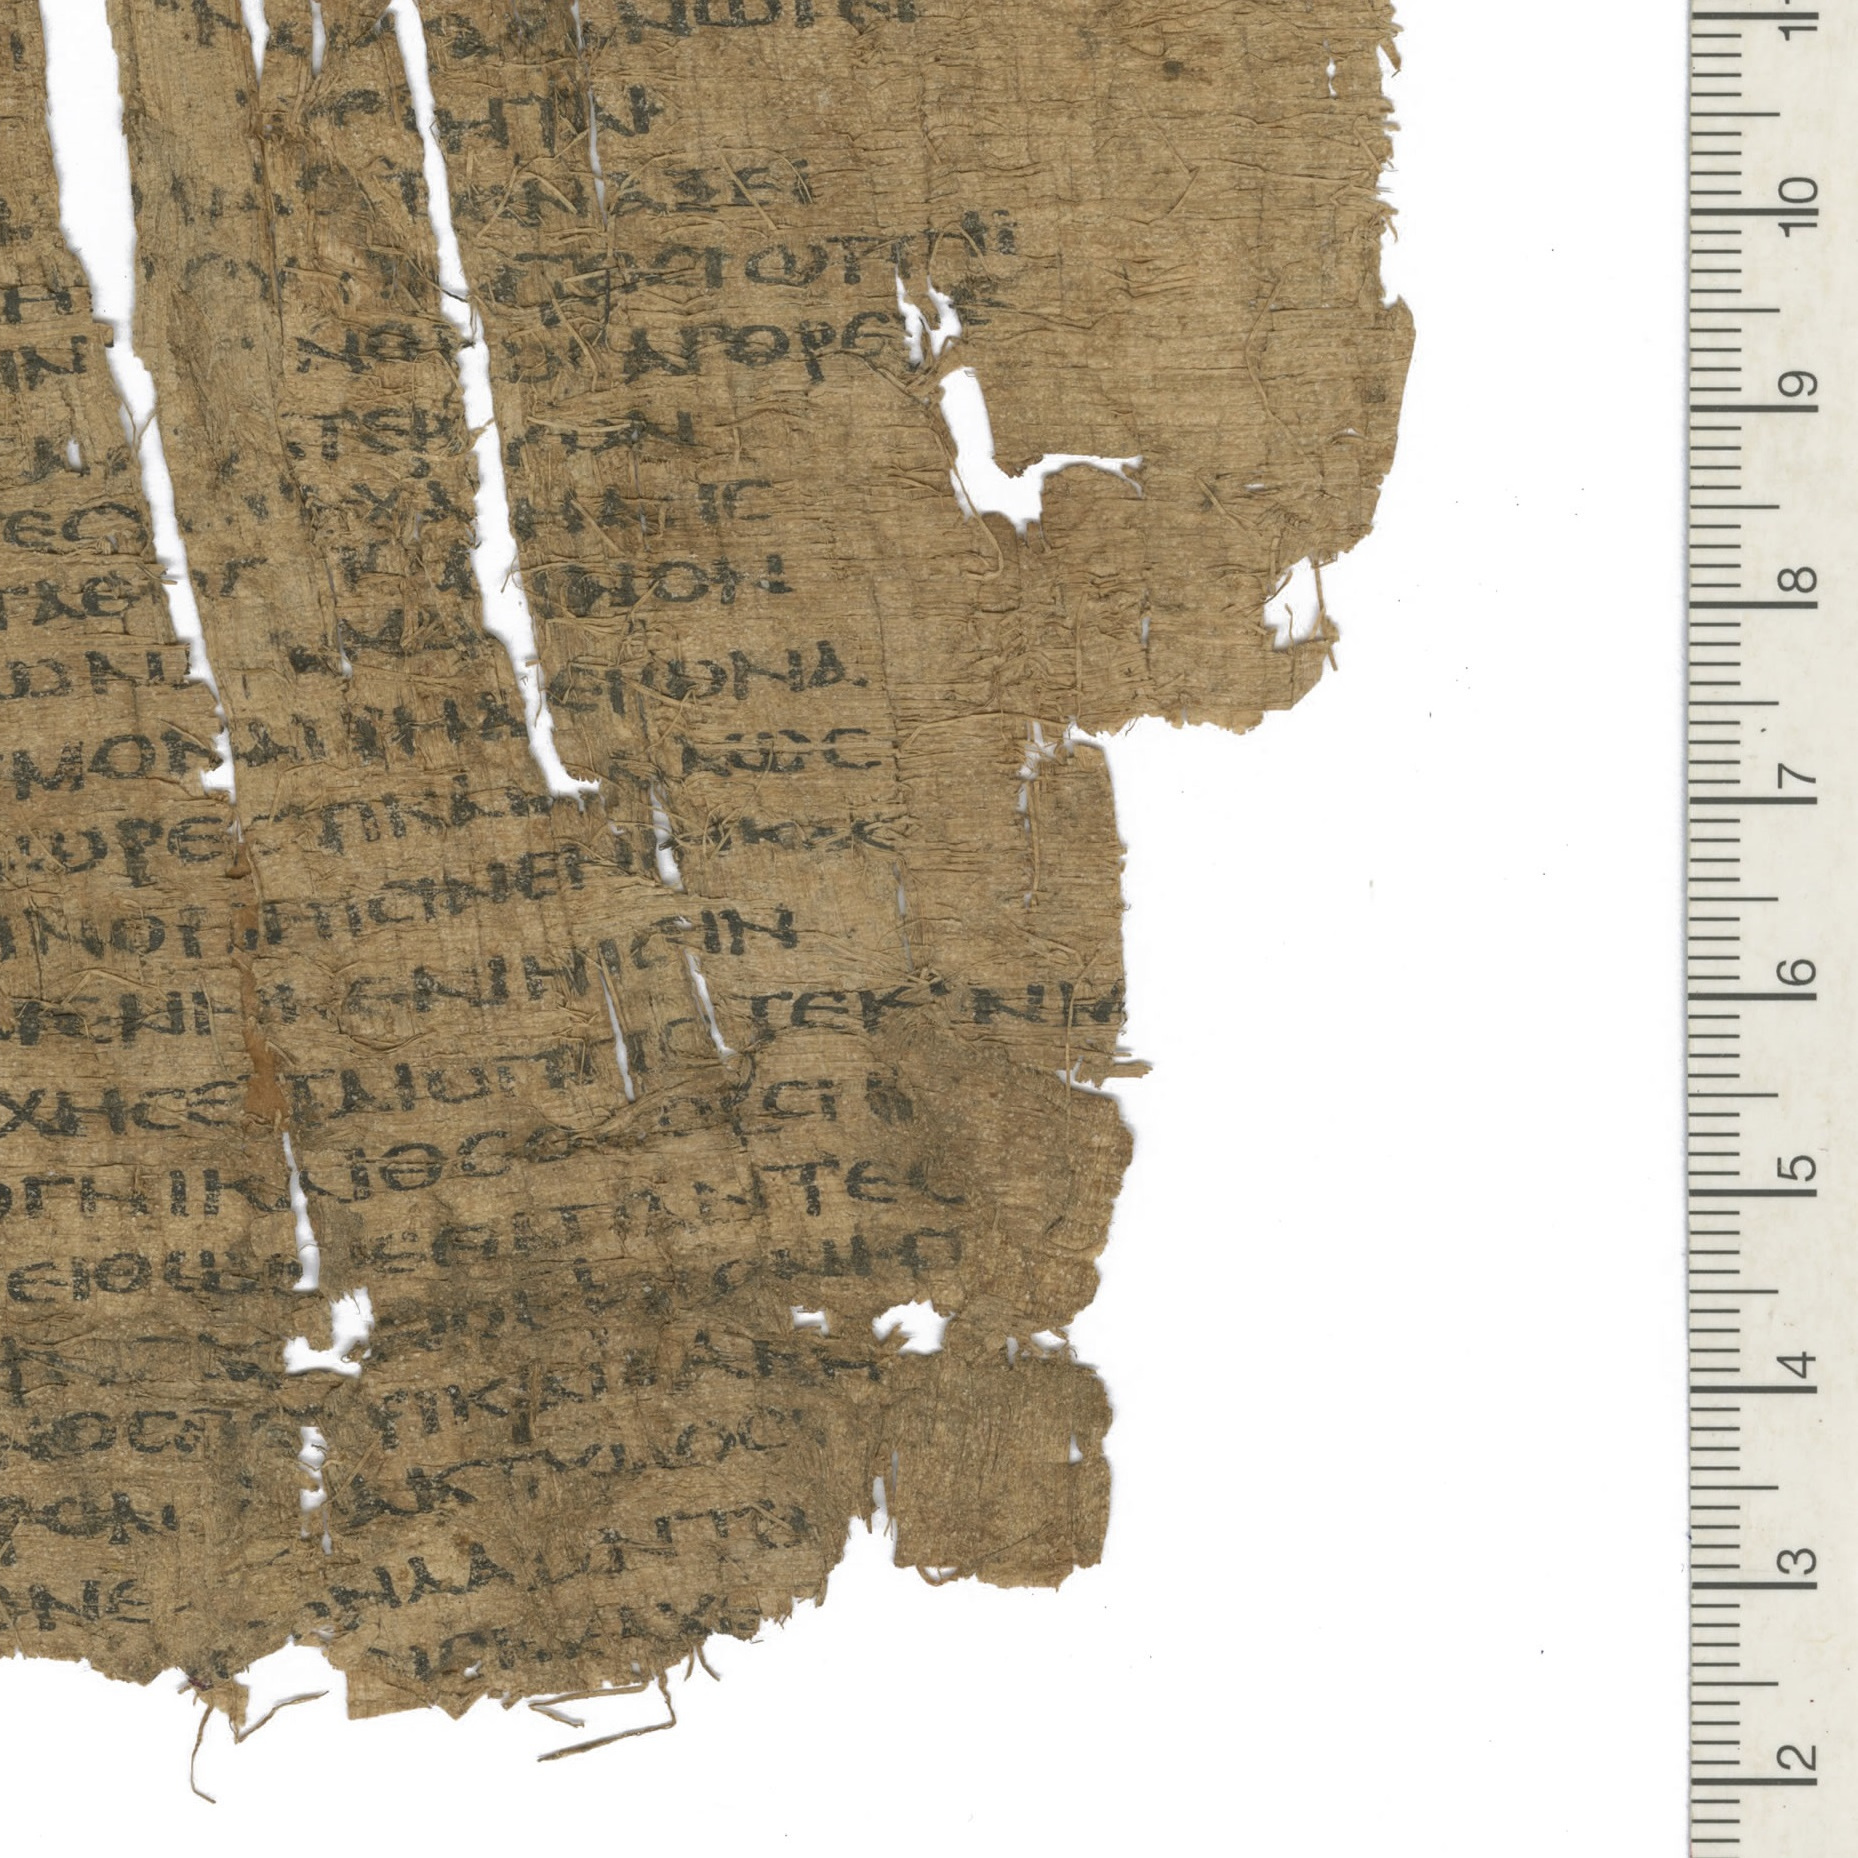
\includegraphics[width=\textwidth]{{raw/PSI_XIV_1377r_crop.jpg}}
        \end{subfigure}
    \end{center}
    The four images used to assess binarization methods, cropped to squares so that are easy to tile to make it easy to assess visually.
\end{figure}

\subsection{Evaluation of Methods}

The results of k-means clustering on the evaluation images are included for reference \seefig{binarizationClustering}. These images clearly show that the signal to noise ratio is far too high to be utilized as the general binarization solution for the pipeline, as the signal to noise ratio is sometimes less than $1$.

The results generated by clustering can be directly compared to those of a neural network to see how poor they are. The results generated by DP-Linknet \seefig{binarizationCNN} are visibly much better at including whole glyphs and less of the noise included in the image, especially the papyrus noise.

Using the results of the Gabor wavelet approximation \seefig{binarizationGabor}, a binary mask can be created \seefig{binarizationGaborBinary} using DP-Linknet. This works using the assumption that large amounts of noise in the binary images generated by DP-Linknet are due to intentionally added objects in the original images, which are often more regular in color or shape than the glyphs, which means the Gabor filtered images do not lose this noise, allowing the CNN to pick up on this information to create an image that can be used as a mask to remove these details from the final binarizations \seefig{binarizationMaskedCNN}.

\begin{figure}[H]
    \caption{Four Example Binarizations Generated with Clustering}
    \label{fig:binarizationClustering}
    \begin{center}
        \begin{subfigure}[b]{0.45\textwidth}
            \centering
            \caption{Example File A}
            
\includegraphics[width=\textwidth]{{binarization/clustering/G_02317_26742_Pap_crop.png}}
        \end{subfigure}
        \hfill
        \begin{subfigure}[b]{0.45\textwidth}
            \centering
            \caption{Example File B}
            \includegraphics[width=\textwidth]{{binarization/clustering/G_26734_c_crop.png}}
        \end{subfigure}
        \vfill
        \begin{subfigure}[b]{0.45\textwidth}
            \centering
            \caption{Example File C}
            \includegraphics[width=\textwidth]{{binarization/clustering/P_Hamb_graec_665_crop.png}}
        \end{subfigure}
        \hfill
        \begin{subfigure}[b]{0.45\textwidth}
            \centering
            \caption{Example File D}
            \includegraphics[width=\textwidth]{{binarization/clustering/PSI_XIV_1377r_crop.png}}
        \end{subfigure}
    \end{center}
    The four images were used to assess binarization methods, binarized using k-means with $k=5$. Image A has a near zero signal to noise ratio. Image B has a much better signal to noise ratio for the glyphs, but also contains text that should not be included near the bottom of the image. Images C and D also contain glyph signal, but are both noisy around the glyphs and include non-glyph information such as a ruler in Image D and the border and color scale in image C.
\end{figure}

\begin{figure}[H]
    \caption{Four Example Binarizations Generated with DP-Linknet}
    \label{fig:binarizationCNN}
    \begin{center}
        \begin{subfigure}[b]{0.45\textwidth}
            \centering
            \caption{Example File A}
            
\includegraphics[width=\textwidth]{{binarization/cnn/G_02317_26742_Pap_crop.png}}
        \end{subfigure}
        \hfill
        \begin{subfigure}[b]{0.45\textwidth}
            \centering
            \caption{Example File B}
            \includegraphics[width=\textwidth]{{binarization/cnn/G_26734_c_crop.png}}
        \end{subfigure}
        \vfill
        \begin{subfigure}[b]{0.45\textwidth}
            \centering
            \caption{Example File C}
            \includegraphics[width=\textwidth]{{binarization/cnn/P_Hamb_graec_665_crop.png}}
        \end{subfigure}
        \hfill
        \begin{subfigure}[b]{0.45\textwidth}
            \centering
            \caption{Example File D}
            \includegraphics[width=\textwidth]{{binarization/cnn/PSI_XIV_1377r_crop.png}}
        \end{subfigure}
    \end{center}
    The four images used to assess binarization methods, binarized using DP-Linknet \cite{Xiong} with  confidence value of 2. Image A has clearly defined glyphs, especially when compared to the results of clustering. Image B has a similar signal to noise ratio for the glyphs to the clustering, with the extra text near the bottom of the image still being included. Images C and D also contain glyph signal, and are less noisy around the glyphs and include non-glyph information such as a ruler in Image D and the border and color scale in image C.
\end{figure}

\begin{figure}[H]
    \caption{Four Example Gabor Filtered Images}
    \label{fig:binarizationGabor}
    \begin{center}
        \begin{subfigure}[b]{0.45\textwidth}
            \centering
            \caption{Example File A}
            
\includegraphics[width=\textwidth]{{binarization/gabor/G_02317_26742_Pap_crop.png}}
        \end{subfigure}
        \hfill
        \begin{subfigure}[b]{0.45\textwidth}
            \centering
            \caption{Example File B}
            \includegraphics[width=\textwidth]{{binarization/gabor/G_26734_c_crop.png}}
        \end{subfigure}
        \vfill
        \begin{subfigure}[b]{0.45\textwidth}
            \centering
            \caption{Example File C}
            \includegraphics[width=\textwidth]{{binarization/gabor/P_Hamb_graec_665_crop.png}}
        \end{subfigure}
        \hfill
        \begin{subfigure}[b]{0.45\textwidth}
            \centering
            \caption{Example File D}
            \includegraphics[width=\textwidth]{{binarization/gabor/PSI_XIV_1377r_crop.png}}
        \end{subfigure}
    \end{center}
    The four images used to assess binarization methods, passed through the Gabor wavelet approximation function.
\end{figure}

\begin{figure}[H]
    \caption{Four Example Gabor Wavelet Binarized Images}
    \label{fig:binarizationGaborBinary}
    \begin{center}
        \begin{subfigure}[b]{0.45\textwidth}
            \centering
            \caption{Example File A}
            
\includegraphics[width=\textwidth]{{binarization/gaborMask/G_02317_26742_Pap_crop.png}}
        \end{subfigure}
        \hfill
        \begin{subfigure}[b]{0.45\textwidth}
            \centering
            \caption{Example File B}
            \includegraphics[width=\textwidth]{{binarization/gaborMask/G_26734_c_crop.png}}
        \end{subfigure}
        \vfill
        \begin{subfigure}[b]{0.45\textwidth}
            \centering
            \caption{Example File C}
            \includegraphics[width=\textwidth]{{binarization/gaborMask/P_Hamb_graec_665_crop.png}}
        \end{subfigure}
        \hfill
        \begin{subfigure}[b]{0.45\textwidth}
            \centering
            \caption{Example File D}
            \includegraphics[width=\textwidth]{{binarization/gaborMask/PSI_XIV_1377r_crop.png}}
        \end{subfigure}
    \end{center}
    The four images used to assess binarization methods, passed through the Gabor wavelet approximation function and then passed through DP-Linknet to create a rudimentary mask that contains some non-glyph information.
\end{figure}

\begin{figure}[H]
    \caption{Four Example CNN Binarized Images (Masked)}
    \label{fig:binarizationMaskedCNN}
    \begin{center}
        \begin{subfigure}[b]{0.45\textwidth}
            \centering
            \caption{Example File A}
            
\includegraphics[width=\textwidth]{{binarization/cnnMasked/G_02317_26742_Pap_crop.png}}
        \end{subfigure}
        \hfill
        \begin{subfigure}[b]{0.45\textwidth}
            \centering
            \caption{Example File B}
            \includegraphics[width=\textwidth]{{binarization/cnnMasked/G_26734_c_crop.png}}
        \end{subfigure}
        \vfill
        \begin{subfigure}[b]{0.45\textwidth}
            \centering
            \caption{Example File C}
            \includegraphics[width=\textwidth]{{binarization/cnnMasked/P_Hamb_graec_665_crop.png}}
        \end{subfigure}
        \hfill
        \begin{subfigure}[b]{0.45\textwidth}
            \centering
            \caption{Example File D}
            \includegraphics[width=\textwidth]{{binarization/cnnMasked/PSI_XIV_1377r_crop.png}}
        \end{subfigure}
    \end{center}
    The four images used to assess binarization methods, binarized using DP-Linknet \cite{Xiong} with  confidence value of 2 and then masked by the binarizations of the Gabor filtered images with the removed black parts of the image shown in grey. No changes were made to image A, as there was no detail that the CNN could recognize left in the Gabor filtered image. The extra text from image B is mostly removed, with the glyph information intact. Similarly, images C and D have their glyph information intact, with the artificial noise in the image being partially removed.
\end{figure}

% \subsection{BiNet}
% \todo{TODO: ADD CONTENT}

\section{Glyph Bounding}

\subsection{Evaluation Metrics}
\todo{NEW}

As the ground-truth information provided for bounding boxes are not tight, perfectly accurate metrics on bounding are not possible without manually tightly rebounding each glyph. Therefore, IOU is used, along with glyph precision and recall measuring the approximate efficacy of methods, with the caveat that a method may have a lower IOU if it generates tighter bounding boxes than if the bounding box was less tight.

Precision and recall are measured not on pixels, but on glyphs. A prediction is defined as a match tp a truth bounding box if the IOU between the two bounding boxes is greater than zero with each truth bounding box being paired with the prediction bounding box with the highest IOU value. The mean IOU is also recorded for all true positives as a method to determine how close the prediction bounding boxes are to the ground truth values.

\begin{figure}[H]
    \caption{Test Results for Glyph Bounding Methods}
    \label{fig:boundingEval}
    \centering
    \begin{tabular}{ | c | c | c | c | c | }
        \hline
        Bounding Method & Precision & Recall & F1 Score & Mean IOU \\
        \hline
        Connected Components (CC) & 0.2006 & 0.8923 & 0.3276 & 0.3182 \\
        CC w/ Best Cleaning & 0.2335 & 0.8093 & 0.3624 & 0.3142 \\
        \hline
    \end{tabular}
\end{figure}

\subsection{Connected Components}
\todo{NEW}

Glyph bounding using connected components fails to precisely generate bounding boxes due to the flaws in the binarization methods used. Otherwise, the method can tightly bound boxes with a high amount of recall. By removing regions that with centroids in other regions or by removing regions fully inside other regions (which includes the before method), the precision and F1 score can be increased, at the cost of recall \seefig{ccBoundingEval}.

\begin{figure}[H]
    \caption{Test Results for Connected Component Bounding and Cleaning}
    \label{fig:ccBoundingEval}
    \centering
    \begin{tabular}{ | c | c | c | c | c | }
        \hline
        Cleaning Method & Precision & Recall & F1 Score & Mean IOU \\
        \hline
        None & 0.2006 & 0.8923 & 0.3276 & 0.3182 \\
        Internal Centroid Removal & 0.2256 & 0.8124 & 0.3531 & 0.3145 \\
        Internal Region Removal & 0.2335 & 0.8093 & 0.3624 & 0.3142 \\
        \hline
    \end{tabular}
\end{figure}

\subsection{Region-Based Convolution Neural Networks}
\todo{NEW}

YOLO, when trained on color images, performs better than when trained on binarized images. In addition, by training YOLO to recognize all glyphs as one class instead of each glyph class as its own class increases accuracy \seefig{evalYOLORaw}. In addition, networks were trained with and without freezing the backbone layers, which are the layers defined as the initial convolutional layers (layers 0-9) \cite{YoloBackbone} that process the input before the main convolutions are performed. This allowed for faster training with a potential for lost accuracy.

\textit{The accuracy metrics taken for each YOLO model were generated on the evaluation set to ensure that the final test set evaluation could be done on unseen data. Therefore, the classification metrics in this sub-section will not map directly to the results of the same classification methods when utilized in the final pipeline.}

\begin{figure}[H]
    \caption{Evaluation Results for YOLO Bounding}
    \label{fig:evalYOLORaw}
    \centering
    \begin{tabular}{ | c | c | c | c | c | }
        \hline
        Training Set & Backbone Layers & Image Type & Model Size & F1 Score \\
        \hline
        Multi-Class & Frozen & Color & YOLOv5x (largest) & 0.07 \\
        Mono-Class & Frozen & Binary & YOLOv5l (large) & 0.63 \\
        Mono-Class & Frozen & Color & YOLOv5l (large) & 0.68 \\
        Mono-Class & Frozen & Color & YOLOv5x (largest) & 0.69 \\
        Mono-Class & Unfrozen & Color & YOLOv5x (largest) & 0.74 \\
        Mono-Class & Unfrozen & Color & YOLOv5x (largest) & 0.72* \\
        \hline
    \end{tabular}
    *All the models were trained for 300 epochs, with the exception of this one, which was trained for 600 epochs, with the metrics being taken on only the last 300 epochs.
\end{figure}

\subsubsection{RCCN Sliding Window}
\todo{TODO: Dec 09}

By introducing a sliding window to the

\subsubsection{RCNN Duplicate Removal}
\todo{TODO: Dec 09}

\subsubsection{Binarization-Assisted CNN}
\todo{TODO: Dec 09}

\section{Line Bounding}
\todo{NEW}

As in glyph bounding, no ground truth information was provided for which glyphs where in the same line, so a visual approximation must be used to determine which methods are best, at least when comparing results of each metric without taking the rest of the pipeline into account.

\subsection{Point Of Interest Clustering}
\todo{TODO: Dec 11}

\subsection{Adjacent Glyph Clustering}
\todo{TODO: Dec 11}

\subsection{Overlaping Glyph Clustering}
\todo{TODO: Dec 11}

\section{Classification}

\textit{The accuracy metrics taken for the classification methods were generated on the evaluation set to ensure that the final test set evaluation could be done on unseen data. Therefore, the classification metrics in this section will not map directly to the results of the same classification methods when utilized in the final pipeline.}

\subsection{Transfer Learning}
\todo{NEW}

Using the feature vectors generated with AlexNet on the non-NN methods, the best results were obtained using the binarizations of the images generated by DP-Linknet. Using GMMs, Random Forests, and $K$-Nearest Neighbors (k-NN) \seefig{classificationEuclideanNonNN} were generated with the full color and binarized images and Euclidean distance calculations \seeeq{distanceEuclidian}, with the best results for each method being shown, where F1 score is the average of the per-glyph F1 score weighted by glyph class occurrence frequency.

\begin{figure}[H]
    \caption{Evaluation Results for Euclidean Non-NN Transfer Learning Classification}
    \label{fig:classificationEuclideanNonNN}
    \centering
    \begin{tabular}{ | c | c | c | }
        \hline
        Classification Method & Color F1 Score & Binary F1 Score \\
        \hline
        GMM & 0.07 & 0.08 \\
        Random Forest & 0.11 & 0.19 \\
        KNN & 0.08 & 0.14 \\
        \hline
    \end{tabular}
\end{figure}

By generating a new set of training data by training the classifications on exactly one randomly chosen template for each class and footmark type, the results were mostly unchanged, but were significantly increased by manually cleaning the templates to remove noise and other small imperfections in the characters \seefig{classificationKNNTemplates}. These results were generated using only a k-NN classifier as it was the fastest to train and did not require as many example images to train an accurate model. These results show that the k-NN classifier can be trained on very few images and generate comparable results to a dataset that is magnitudes larger, which shows promise for classification on similar problems with significantly less training data.

\begin{figure}[H]
    \caption{Evaluation Results for Templated k-NN Transfer Learning Classification}
    \label{fig:classificationKNNTemplates}
    \centering
    \begin{tabular}{ | c | c | c | c | }
        \hline
        Template Type & Distance & Best $k$ Value & Weighted F1 Score \\
        \hline
        Color & Euclidean & 5 & 0.08 \\
        Cleaned Binary & Euclidean & 5 & 0.27 \\
        Cleaned Binary & Manhattan & 4 & 0.34 \\
        Cleaned Binary & Cosine & 5 & 0.39 \\
        \hline
    \end{tabular}
\end{figure}

Using pretrained neural networks to classify the data generated better results, both on binarized and color images of glyphs \seefig{classificationFeatureVectorNN}. Using these networks a higher classification accuracy was attainable with unaltered training data, producing better results with less manual work being required.

\begin{figure}[H]
    \caption{Evaluation Results for NN Transfer Learning Classification}
    \label{fig:classificationFeatureVectorNN}
    \centering
    \begin{tabular}{ | c | c | c | }
        \hline
        Network & Image Type & Weighted F1 Score \\
        \hline
        Linear & Binary & 0.666 \\
        Linear & Color & 0.626 \\
        Simple-LSTM & Color & 0.593 \\
        LSTM-to-Linear & Color & 0.662 \\
        Linear-to-LSTM & Binary & 0.710 \\
        Linear-to-LSTM & Color & 0.668 \\
        \hline
    \end{tabular}
\end{figure}

\subsection{Convolutional Neural Networks}
\todo{NEW}

Using architectures based on the convolutional layers of AlexNet \cite{Krizhevsky}, ResNeXt \cite{Xie}, and MNIST9975 \cite{Deotte}. The network based on AlexNet generates similar results to those based on the feature vectors generated by AlexNet, but has a higher weighted F1 score. The networks based on ResNext preform even better, at the cost of time, taking much longer to train and evaluate \seefig{classificationCNN}. In these larger, more complex models, the binarized images preformed worse across all the models than the color images, so only the peak color image F1 score is used for evaluation. Each network was trained for approximately $100$ epochs on the same train and evaluation image and word sets.

\begin{figure}[H]
    \caption{Evaluation Results for CNN Classification}
    \label{fig:classificationCNN}
    \centering
    \begin{tabular}{ | c | c | c | }
        \hline
        Base Network & Modified Network Name & Weighted F1 Score \\
        \hline
        AlexNet & Alex LSTM & 0.754 \\
        ResNet50 & ResNet LSTM & 0.786 \\
        ResNext50 & ResNext50 Classify-to-LSTM & 0.700 \\
        ResNext50 & ResNext50 LSTM-To-Dense & 0.835 \\
        ResNext50 & ResNext50 LSTM-To-Dense & 0.836 \\
        ResNext101 & ResNext101 LSTM-Dense & TODO \\
        \hline
    \end{tabular}
\end{figure}

\subsection{Stochastic Language Models}
\todo{TODO: Dec 09}

\todo{talk about uncertainty markov and top n markov}

\subsection{Neural Netork Language Models}
\todo{TODO: Dec 09}

\todo{talk about batchsize vs accuracy on resnet50 and shuffle test}

\section{Pipeline}
\todo{TODO: DEC 14}


\section{Evaluation Metric Analysis}

\subsection{Ground Truth Comparison}
\todo{TODO: Dec 12}

\subsection{Visual Analysis}
\todo{TODO: Dec 12}

\subsection{BLEU Score}
\todo{TODO: Dec 12}
\cite{Callison-Burch}
